\section{$Re_{\tau}=1000$ simulation} 
The second simulation performed is carried out at $Re_{\tau}=1000$, which in terms of channel width and bulk velocity is equivalent to $Re_{b}\approx40000$.\par
The bulk velocity, obtained as shown in~\ref{bulk:velocity}, is 19.99, while $\alpha_{0}$ and $\beta_{0}$ are respectively 0.5 and 1, in order to reproduce the correct dimensions of the channel, as shown in chapter~\ref{chapter:Re180}.\par
Since the high computational cost needed to obtain these results we were unable to carry out a complete simulation. Thus the results reported show the statistics associated with a flow in a transitory state. \\~\par

The simulation employed a variable timestep, determined through the Courant-Friedrichs-Lewy condition. Since its high computational cost, due to the needed transpositions and Fourier transformations, we decided to set the CFL limit below the stability threshold and calculate it once every $n$ steps. In this way the gain in terms of performance is significant, combining the flexibility of the Courant-Friedrichs-Lewy condition with a reduced cost to compute it.\\~\par

The grid employed in this simulation face 500 points in the wall-normal direction, 2048 in the spanwise direction and 2048 points along the streamwise dimension, direction in which we exploit the Hermitian symmetry. According to this configuration, the grid size reach the billion of points.\par
Table~\ref{table:1000} report a summary of the simulation configuration for the $Re_{\tau}=1000$ case.\\~\par

\begin{table}
\caption{Simulation data for $Re_{\tau}$=1000}
\begin{center}
\begin{tabular}{ccccccccccccc}
\toprule
$L_{x}$ & $L_{z}$ & $\delta$ & $nx$ & $nz$ & $ny$ & $\alpha_{0}$ & $\beta_{0}$ & $\Delta x^{+}$ & $\Delta z^{+}$ & $px$ & $CFL$\\
$4\pi$ & $2\pi$ & 1 & 2048 & 2048 & 500 & 0.5 & 1 & 6.1  & 3 & 1 & 1.6 \\
\bottomrule
\end{tabular}
\end{center}
\label{table:1000}
\end{table}


Since are required approximately 50GB of disk space per each field we decided to avoid to save them on disk, instead we calculated the statistics runtime, merging the files at the end of the simulation, reducing the required space to few KB.\\~\par

The results that we will present shortly are obtained through the ensemble average of 100 fields, and cover 0.1 non dimensional time units. In this lapse of time the mean $Re_{\tau}$ is approximately 991 units and it is slowly moving towards the nominal value of the simulation.\par
Let us focus now on the statistics gained from the simulation.\\~\par
Figure~\ref{loglaw:1000} report the law of the wall. As we can see from the plot, made in semi-logarithmic scale using the wall units, our data fits the theoretical curve throughout the logarithmic region, while, towards the centerline, a residual sensitivity to the initial conditions is still present and lead to few differences with the results obtained by Moser \& Lee in~\cite{Lee}.\par
Far from the wall, the velocity defect law shows acceptable agreement with our results, as figure~\ref{velocity:defect:1000} exhibit.\\~\par

\begin{figure}
\begin{center}
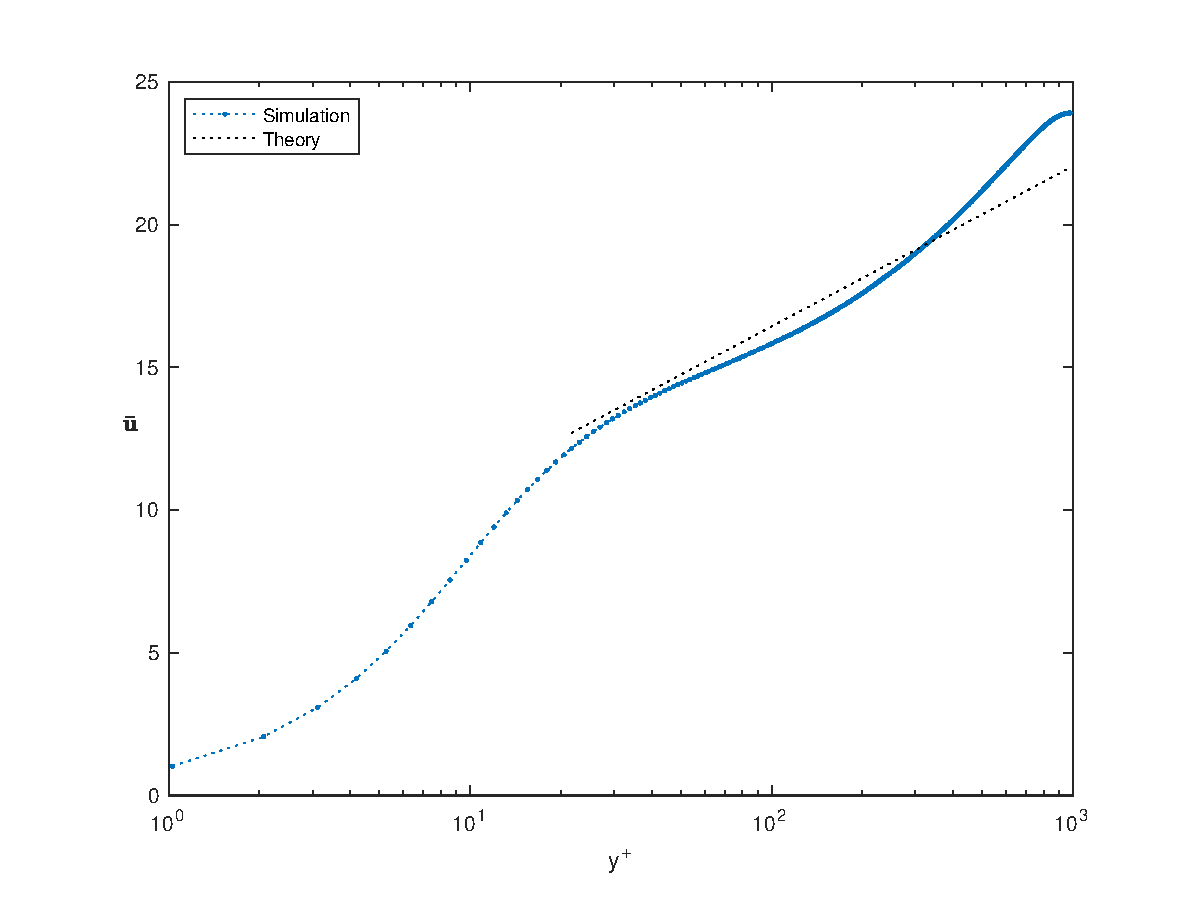
\includegraphics[scale=0.55]{grafici/loglaw_1000.eps}
\caption{$\bar{u}^{+}$ in the near wall region for a $Re_{\tau}=1000$ simulation}
\label{loglaw:1000}
\end{center} 
\end{figure}

\begin{figure}
\begin{center}
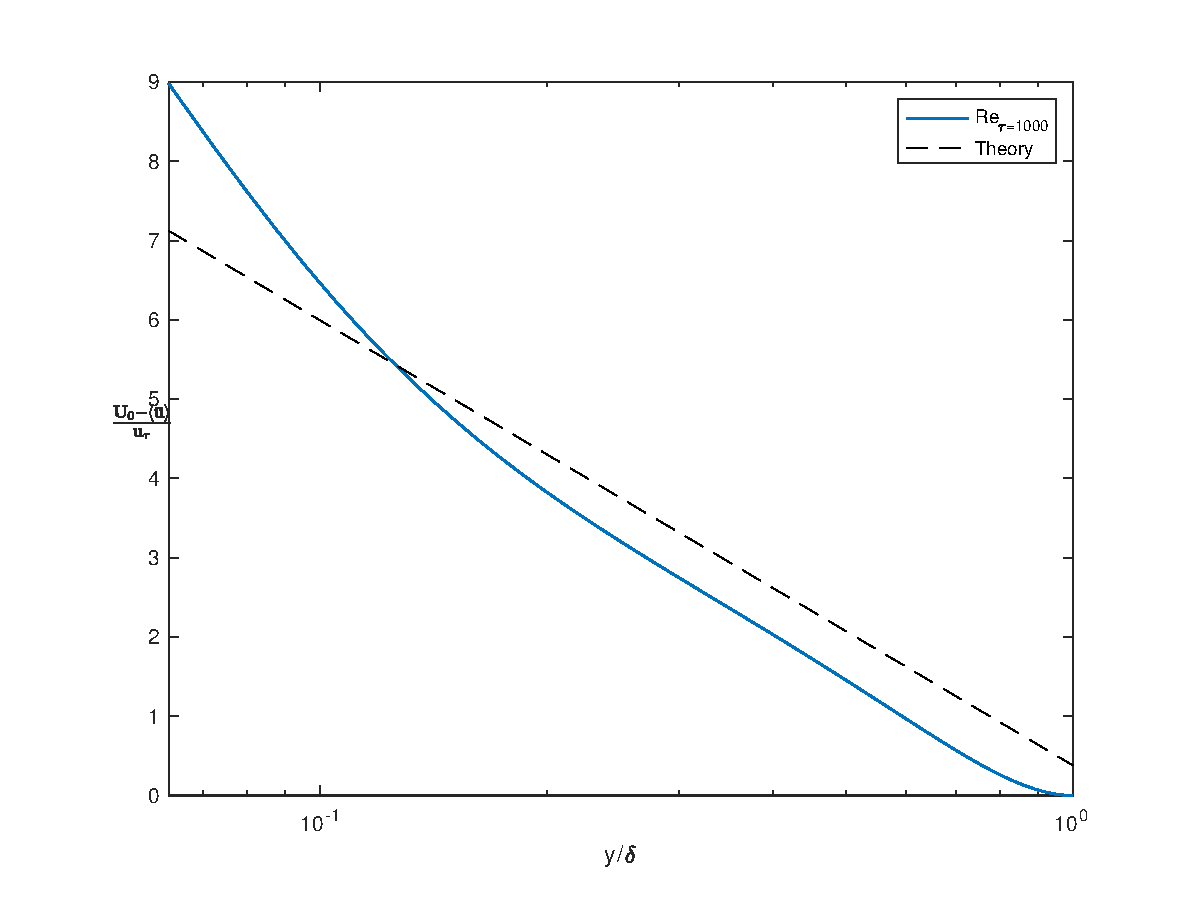
\includegraphics[scale=0.55]{grafici/velocity_defect_1000.eps}
\caption{Velocity defect for a $Re_{\tau}=1000$ simulation}
\label{velocity:defect:1000}
\end{center} 
\end{figure}

In figure~\ref{budget:1000} we reported the \emph{rms} fluctuations, normalized by the $u_{\tau}^{2}$, jointed with the TKE distribution. The first differences that we can immediately face by comparing our curves with the ones in figure~\ref{k+budgets:180} are the peak values. These values tends to increase with respect to the counterpart of the $Re_{\tau}=180$ simulation, highlighting how this simulation contains more energy than the previous ones.\par
Although there is an higher content of energy, the curves shape remains aligned with the ones seen in the previous chapter.\par
The near-wall behavior present a two-components turbulent flow. In fact, as evidenced by the magnification, the wall-normal fluctuations are absent for the first few units.
\\~\par

\begin{figure}
\begin{center}
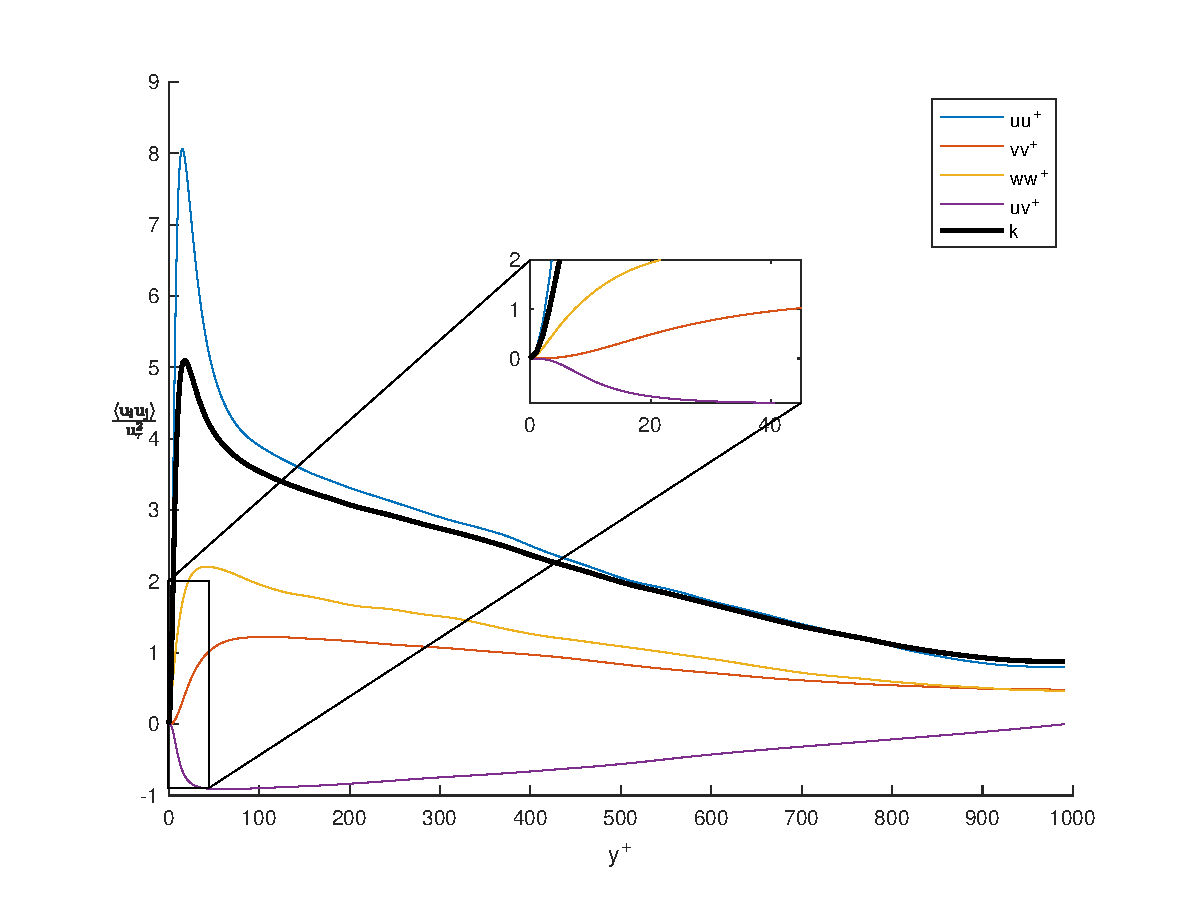
\includegraphics[scale=0.55]{grafici/budget+k_1000.eps}
\caption{\emph{rms} terms for a $Re_{\tau}=1000$ simulation}
\label{budget:1000}
\end{center} 
\end{figure}


The finer mesh and the higher Reynolds evidenced the appearance of a new turbulence peak, detached from the wall-cycle, identified through knees in the curves of figure~\ref{rms:1000}. \par
In such figure our results are compared with the ones of Moser \& Lee, which are the expected values for a complete $Re_{\tau}=1000$ simulation. \par
The results shows accordance among the expected values and the ones obtained through the simulation.
The $u'/u_{\tau}$ curve fits well the expect value, despite the little $Re_{\tau}$ difference among the two datasets.
The $v'/u_{\tau}$ and $w'/u_{\tau}$ curves are in good accordance with the values of Moser \& Lee in the inner region, while towards the centerline of the channel flow we face the raise of differences, possibly due to the transitory nature of the simulation and the dependency on the initial conditions.\\~\par

\begin{figure}
\begin{center}
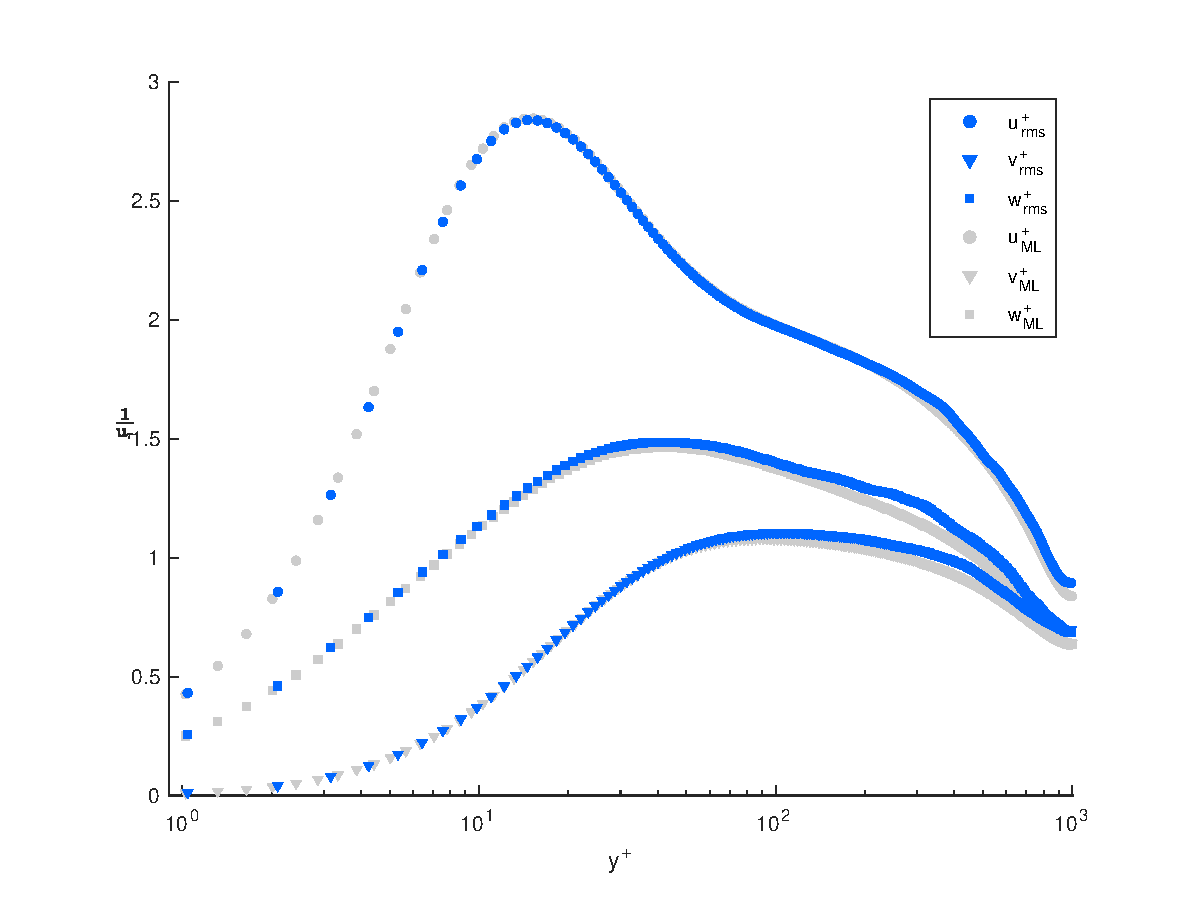
\includegraphics[scale=0.55]{grafici/rms_1000.eps}
\caption{\emph{rms} behavior on a $Re_{\tau}=1000$ simulation}
\label{rms:1000}
\end{center} 
\end{figure}

Comparing the results of this simulation with the ones of the $Re_{\tau}=180$ we can clearly see a generalized upward shift of the \emph{rms} fluctuations. Such trend is present also near the wall. Indeed the curves does not exhibit marked changes in shape with respect to their counterpart in the previous simulation, as figure~\ref{wall:rms:1000} testify, just an upward shift, with the streamwise and spanwise components that depart from zero as $y^{+}$, while the wall-normal components leave the wall as $y^{2+}$. \\~\par

Similar reasoning applies also for the graphs of the \emph{production}, reported in figure~\ref{tke:prod:1000}, that reach a slightly higher peak of $P/Re_{\tau}=0.24$, without showing significant changes of the curve shape. The peak is still located nearby $y\approx 12$.\\~\par

As theory affirms, the wall coordinate of the peak of production corresponds to that in which the stress components become equivalent. This aspect will be investigated further, comparing the results of the two simulations together.
At the present time we limit to illustrate the behavior of the stress components, which are reported in figure~\ref{stresses:1000}. As we can see, the normalized total shear stress is quasi-straight, suggesting that we are still in a transitory phase. The driving-train of this unsteadiness has to be searched in the excess of Reynolds stresses, which are forcing our flow towards higher Reynolds values. \par
\begin{figure}
\begin{center}
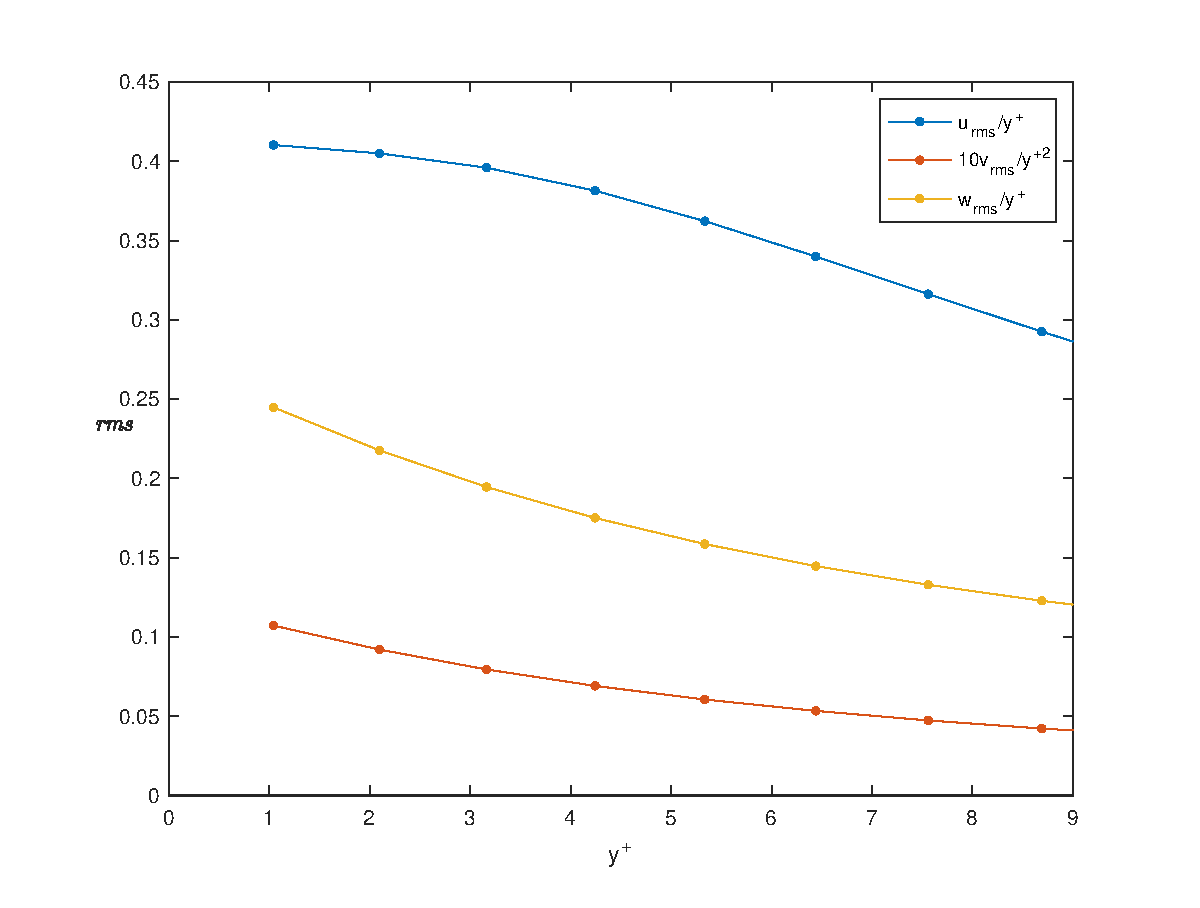
\includegraphics[scale=0.55]{grafici/wall_rms_1000.eps}
\caption{Normalized \emph{rms} close to the wall for a $Re_{\tau}=1000$ simulation}
\label{wall:rms:1000}
\end{center} 
\end{figure}

\begin{figure}
\begin{center}
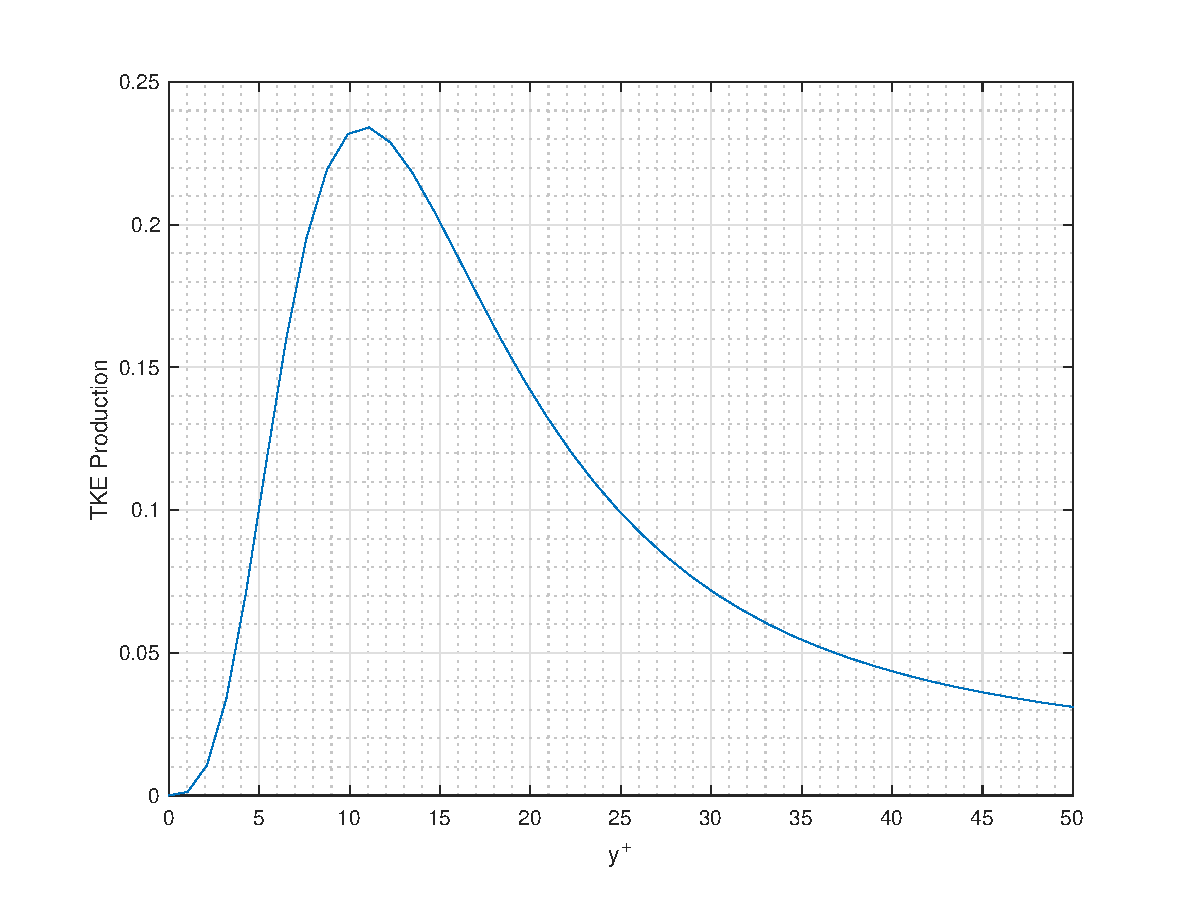
\includegraphics[scale=0.55]{grafici/tke_prod_1000.eps}
\caption{Production term of the TKE eq. for a $Re_{\tau}=1000$ simulation}
\label{tke:prod:1000}
\end{center} 
\end{figure}

\begin{figure}
\begin{center}
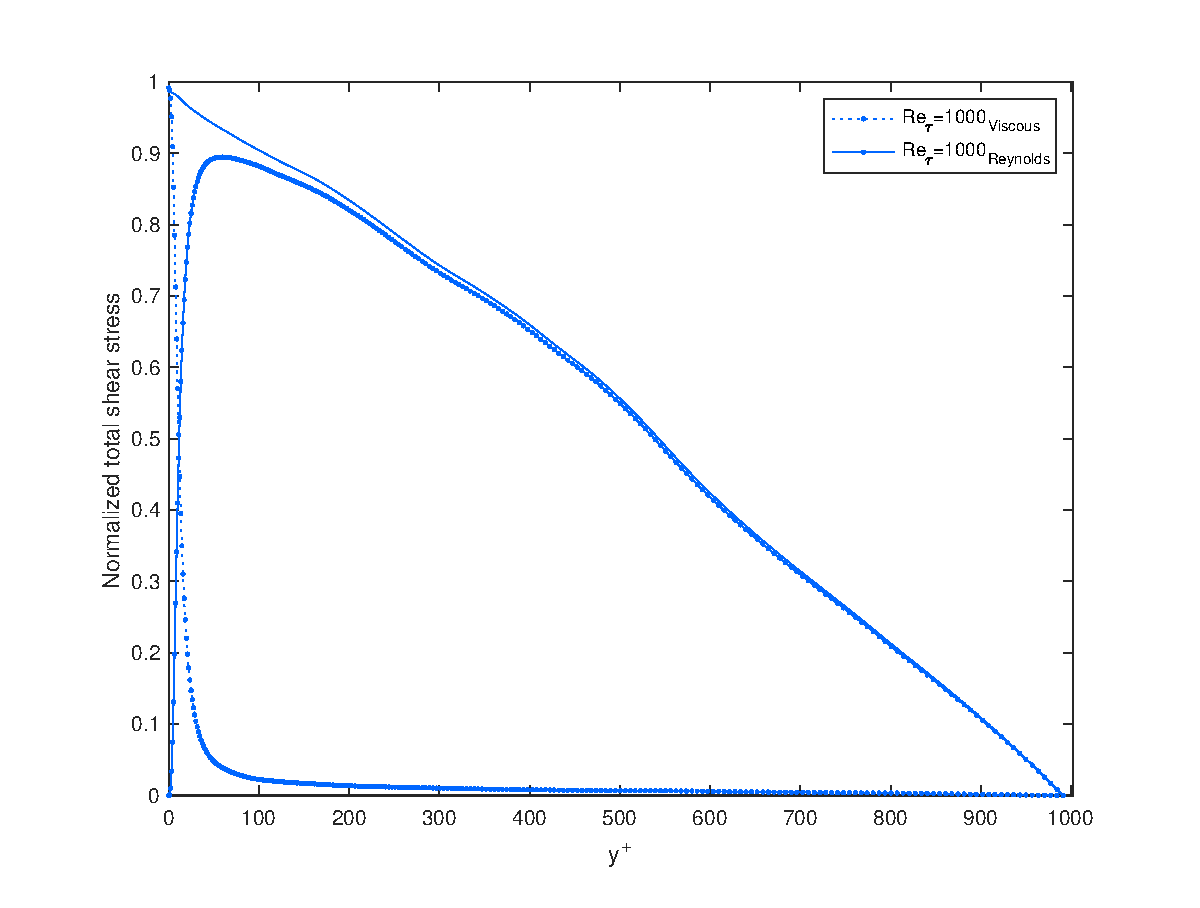
\includegraphics[scale=0.55]{grafici/stresses_1000.eps}
\caption{Normalized total shear stress for a $Re_{\tau}=1000$ simulation}
\label{stresses:1000}
\end{center} 
\end{figure}